
%(BEGIN_QUESTION)
% Copyright 2015, Tony R. Kuphaldt, released under the Creative Commons Attribution License (v 1.0)
% This means you may do almost anything with this work of mine, so long as you give me proper credit

Denne produksjonsprosessen produserer {\it ammoniumnitrat}, en hovedbestanddel i kunstgjødsel, ved kjemisk kombinasjon av salpetersyre og ammoniakk:

$$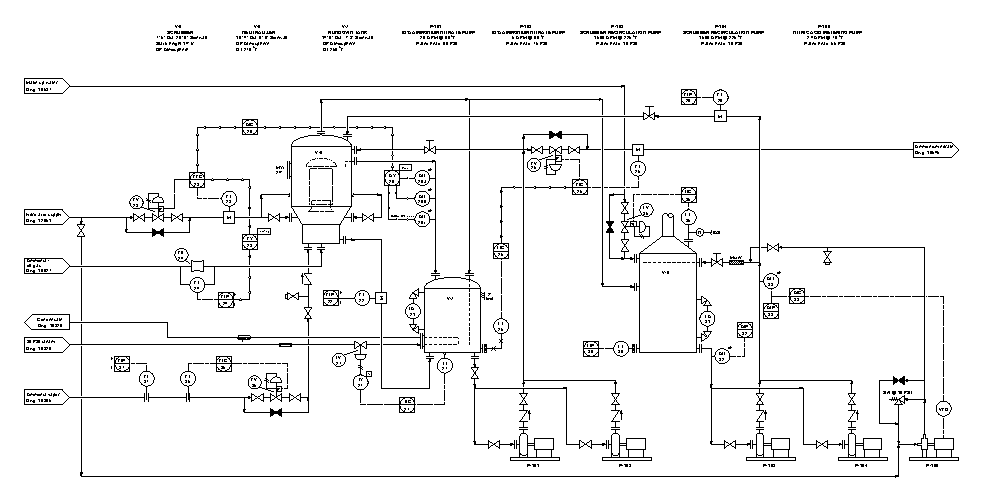
\includegraphics[width=15.5cm]{i0008rx01.eps}$$

Undersøk nivåreguleringssystemet for runoff-tanken (V-7), og identifiser en av lastene i denne reguleringssløyfen. Etter at du har identifisert lasten, legg til en transmitter som måler denne lastvariabelen, og legg til nødvendige reguleringsfunksjoner for å implementere en {\it feedforward}-strategi for nivåreguleringen i runoff-tanken.

\underbar{file i01276}
%(END_QUESTION)





%(BEGIN_ANSWER)

Kanskje den viktigste lasten i nivåreguleringssløyfen for runoff-tanken er innkommende flow fra nøytraliseringsbeholderen (V-6) gjennom linjen med de tre pH-transmitterne, siden endringer i denne flowen vil få nivåregulatoren (LIC-26) til å korrigere for å holde nivået ved setpunkt.

\vskip 10pt

Feedforward-transmitteren for denne lasten vil naturligvis være en flowtransmitter plassert i linjen som fører ammoniumnitrat fra V-6 til V-7. Signal fra denne transmitteren vil gå gjennom en gain/bias-funksjon og deretter (eventuelt) gjennom en lead/lag-funksjon før det går inn i en summer-funksjon plassert mellom LIC-26 og FIC-25. På denne måten legges det proporsjonerte feedforward-signalet til det kaskadekoblede setpunktet til FIC-25, som krever mer eller mindre utløpsflow fra V-7 i samsvar med hvor mye flow som går inn i V-7 fra V-6.
 
%(END_ANSWER)





%(BEGIN_NOTES)


%INDEX% Control, strategies: feedforward
%INDEX% Process: ammonium nitrate production (realistic P&ID shown)

%(END_NOTES)

